\documentclass[12pt,a4paper]{report}
\usepackage[utf8]{inputenc}
\usepackage[english,russian]{babel}
\usepackage{indentfirst}
\usepackage{pdfpages}
\usepackage{titlesec}
\usepackage{listings}
\usepackage{amsmath}
\usepackage{float}

% Вставка картинки
\usepackage{graphicx}
\graphicspath{{schemes/}}
\DeclareGraphicsExtensions{.pdf,.png,.jpg}

\usepackage[14pt]{extsizes}

\newcommand{\hsp}{\hspace{20pt}}
\titleformat{\chapter}[hang]{\large\bfseries}{\thechapter{. }}{0pt}{\large\bfseries}
\titlelabel{hlabel-formati}
\titlespacing{\chapter}{42pt}{-20pt}{12pt}
\titleformat{\section}[hang]{\large\bfseries}{\thesection{. }}{0pt}{\large\bfseries}
\titlespacing{\section}{42pt}{12pt}{5pt plus 5pt}

% Отступ абзаца
\usepackage{indentfirst}
\setlength{\parindent}{1.5cm}

% Межстрочный интервал
\usepackage{setspace}
\onehalfspacing % интервал 1.5

\usepackage[left=3cm, right=1cm, top=2cm, bottom=2cm]{geometry}

\begin{document}
% Титульник
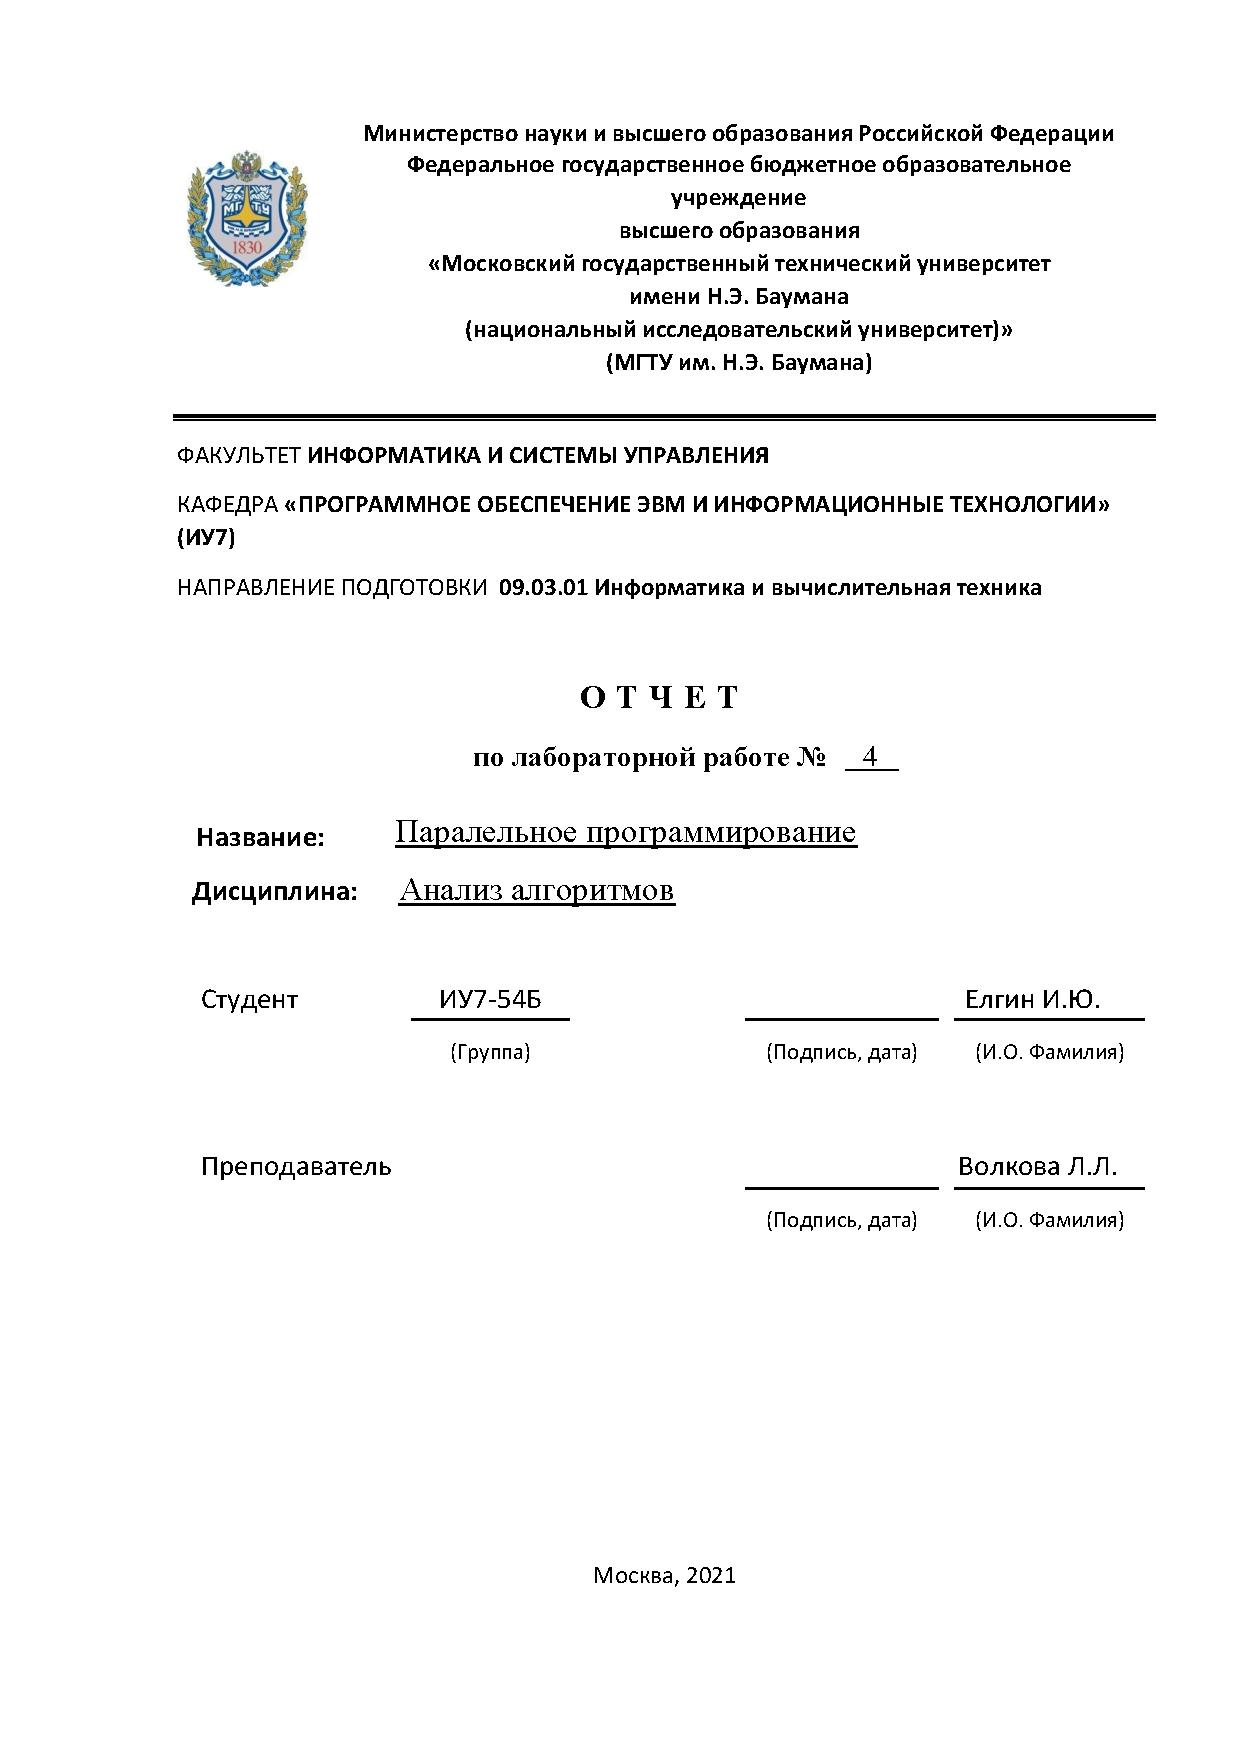
\includepdf[pages=1]{titul.pdf}
% Оглавление
\tableofcontents

\newpage
\chapter*{Введение}
\addcontentsline{toc}{chapter}{Введение}

В данной лабораторной работе реализуется и оценивается параллельный алгоритм поиска наиболее похожего слова с использованием алгоритма Дамерау-Левенштейна.

Параллелизм -- выполнение нескольких вычислений в различных потоках. 
При параллельном программировании в процессоре с многоядерной архитектурой несколько процессов могут выполнятся 
одновременно на разных ядрах.
Это приводит к тому, что время выполнения параллельного алгоритма может быть ощутимо меньше, чем у его 
однопоточного аналога. Однако, на создание потоков тратится время, в связи с чем на малых данных простой алгоритм может показывать лучшие результаты по времени.

Стандартный алгоритм поиска наиболее похожего слова в словаре сводится к проходу по всему словарю и применению алгоритма Дамерау-Левенштейна для введёного слова и очередного слова из словаря. Наименьший результат указывает на наиболее похожее слово в словаре. 

Сравнение очередного слова из словаря с введёным является отдельной процедурой и не зависит от других сравнений. Поэтому мы можем разбить словарь на участки и запустить для них потоки.

\newpage
\chapter{Аналитическая часть}

Целью лабораторной работы является разработка и исследование параллельных алгоритмов поиска наиболее похожего слова в словаре. \\

Можно выделить следующие задачи лабораторной работы:
\begin{itemize}
    \item описание алгоритма поиска похожего слова в словаре;
    \item распаралеливание данного алгоритма;
    \item проведение замеров процессорного времени работы алгоритмов при различном количестве потоков;
    \item анализ полученных результатов.
\end{itemize}

\section{Описание необходимых операций}

Наиболее подходящим словом будем называть слово из словаря с наименьшим результатом выполнения алгоритма Дамерау-Левенштейна.

Алгоритм Дамерау-Левенштейна вычисляет минимальное количество операций необходимых для получения одного слова из другого.

Операции возможные над словом :


\textbf{Действия обозначаются так:} 
\begin{enumerate}
  	\item D (англ. delete) — удалить;
	\item I (англ. insert) — вставить;
	\item R (replace) — заменить;
	\item M (match) - совпадение;
	\item T (transposition) - транспозиция в алгоритме Дамерау - Левенштейна.
	\label{formula:1}
\end{enumerate}
    
В качестве алгоритма Дамерау-Левенштейна выберем алгоритм с тремя строками в виду его быстродействия и экономии памяти \cite{ll}.

\section{Используемые алгоритмы}

Алгоритм подразумевает проход по словарю и выполнение алгоритма Дамерау-Левенштейна для каждой записи.

Параллелизм может быть достигнут за счёт выделения процессов, которые могут выполнятся независимо друг от 
друга.
В данном случае для каждой записи мы можем независимо вычислить результат Дамерау-Левенштейна.

\section{Вывод}

Результатом аналитического раздела стало определение цели и задач работы, описано понятие операций необходимых для реализации алгоритма.

\newpage
\chapter{Конструкторская часть}

В данном разделе рассмотрим описанные алгоритмы нахождения наиболее похожего слова в словаре с.
\section{Алгоритм Дамерау-Левенштейна}
Схема алгоритма Дамерау-Левенштейна приведена на рисунке 2.1, 2.2.
\begin{figure}[H]
    \center{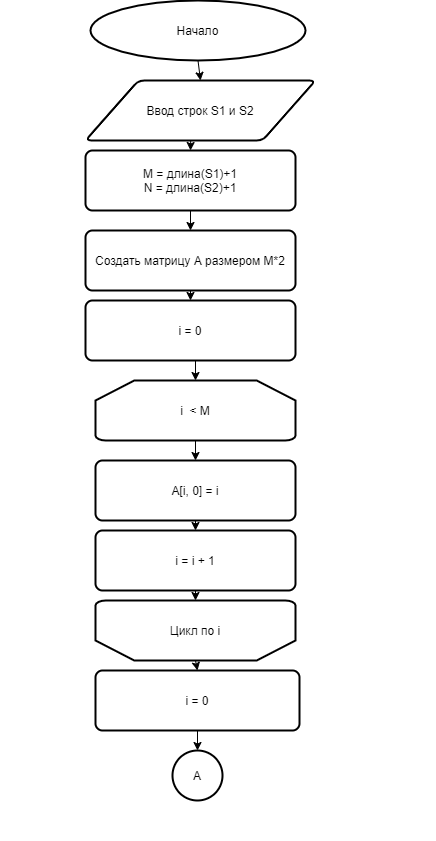
\includegraphics[scale=0.5]{schem/dam1.png}}
    \caption{Схема алгоритма Дамерау-Левенштейна часть 1}
    \label{fig:image}
\end{figure}

\begin{figure}[H]
    \center{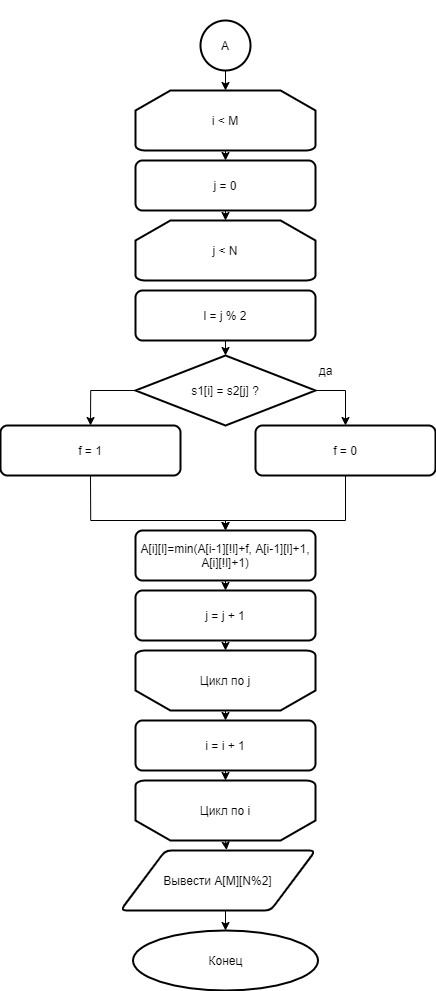
\includegraphics[scale=0.5]{schem/dam2.png}}
    \caption{Схема алгоритма Дамерау-Левенштейна часть 2}
    \label{fig:image}
\end{figure}

\section{Стандартный алгоритм поиска слова}

Схема простого алгоритма приведена на рисунке 2.3.

\begin{figure}[H] 
    \center{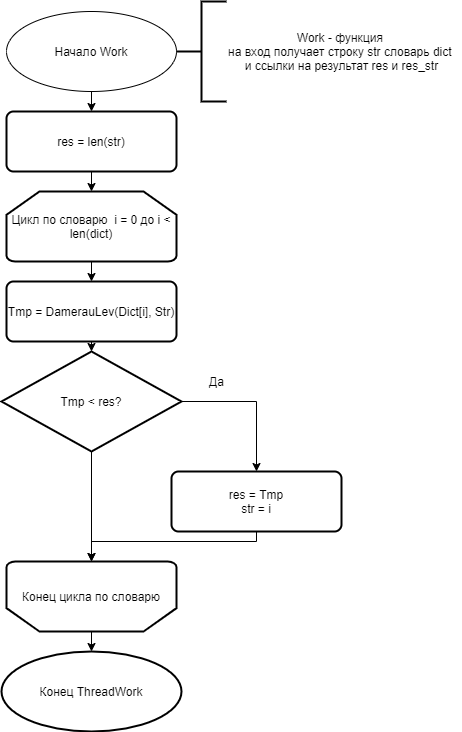
\includegraphics[scale=0.5]{schem/paralel2.png}}
    \caption{Схема простого алгоритма}
    \label{fig:image}
\end{figure}

\newpage
\section{Паралельный алгоритм}

Вычисление значений алгоритма Дамерау-Левенштейна для введёной строки и строк из словаря не зависимо для каждой строки словаря, следовательно может быть распаралелено. 

Пусть производится работа с T потоками а всего записей в словаре N. В таком случае, i-й поток будет производить вычисление с $ (i - 1) * (N / T  + (N - i) \% (N \% T)) $  по $ i * N / T + (N - i) \% (N \% T) $ 
Схема паралельного алгоритма приведена на рисунке 2.4.

\begin{figure}[H]
    \center{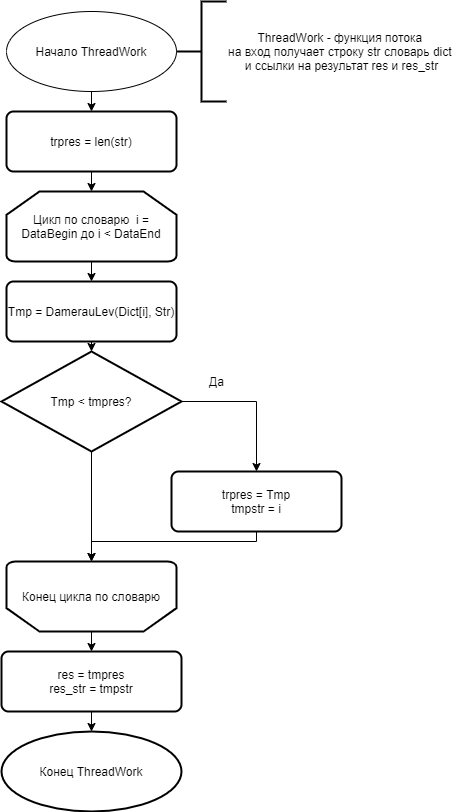
\includegraphics[scale=0.7]{schem/paralel.png}}
    \caption{Схема паралельного алгоритма}
    \label{fig:image}
\end{figure}


\section{Вывод}

Результатом конструкторской части стало схематическое описание алгоритмов поиска наиболее похожего слова в словаре, сформулированы тесты и требования к программному обеспечению.

\newpage
\chapter{Технологическая часть} 
В данной главе происходит выбор языка програмирования и реализация алгоритмов на выбраном языке.
\section{Выбор языка программирования}

В качестве языка программирования был выбран C++, так как имеется опыт работы с ним. Так же для данного языка существуют  
библиотеки, с помощью которых можно удобно создавать потоки. 
 
Разработка проводилась в среде QTCreator.
\section{Реализация потоков}
Потоки реализуются с помощью библиотеки $Threads$ \cite{cpp_info}.

Для избежания неправильных ответов в результате гонок потоков был использован мютекс из библиотеки $Mutex$ \cite{new}.

Для передачи данных в функцию потока была создана структура включающая ссылки на результат, данные обрабатываемые потоком и мьютекс листинг 3.1.
\newpage
\textrm{Листинг 3.1: Структура данных}
\begin{lstlisting}[frame=single, numbers=left]
struct args{
    args(int &result0,int &res_string0,int data_start0,int data_end0,std::vector <std::string> &data0,std::string &serch_str0,std::mutex &mtx0):
        result(result0),
        res_string(res_string0),
        data_start(data_start0),
        data_end(data_end0),
        data(data0),
        serch_str(serch_str0),
        mtx(mtx0)
    {};
    int &result;
    int &res_string;
    int data_start;
    int data_end;
    std::vector <std::string> &data;
    std::string &serch_str;
    std::mutex &mtx;
};
\end{lstlisting}
\section{Листинг кода}

В листингах 3.2 - 3.6 приведены реализации поиска наиболее похожего слова в словаре. \\
\newpage
\textrm{Листинг 3.2: функция алгоритма Дамерау-Левенштейна}
\begin{lstlisting}[frame=single, numbers=left]
int DemLevAlg(std::string &str1, std::string &str2)
{
    int f;
    int l, l1, l2;

    int n = str1.length() + 1, m = str2.length() + 1;

    int matrix[n + 1][3];
    for (int i = 0; i < n; i++)
        matrix[i][0] = i;

    for (int j = 1; j < m; j++)
    {
        l = j % 3;
        l1 = (l + 2) % 3;
        l2 = (l + 1) % 3;
        matrix[0][l] = j;
        for (int i = 1; i < n; i++)
        {
            if (str1[i] == str2[j])
                f = 0;
            else
                f = 1;
            if (i != 1 and j != 1 and str1[i] == str1[j-1] and str2[j] == str1[i-1])
                matrix[i][l] = min(matrix[i-2][l2] + 1, matrix[i-1][l1] + f, matrix[i-1][l] + 1, matrix[i][l1] + 1);
            else
                matrix[i][l] = min(matrix[i-1][l1] + f, matrix[i-1][l] + 1, matrix[i][l1] + 1);
        }
    }
    return matrix[n - 1][(m - 1)%3];
}
\end{lstlisting}
\newpage
\textrm{Листинг 3.3: функция потоков и их создания}
\begin{lstlisting}[frame=single, numbers=left]
void thread_work(args arg)
{	int temp_res = DemLevAlg(arg.data.at(arg.data_start), arg.serch_str), temp_str = arg.data_start;
    int tmp;
    for (int i = arg.data_start; i < arg.data_end; i++)
    {	tmp = DemLevAlg(arg.data.at(i), arg.serch_str);
        if (tmp < temp_res)
        {
            temp_res = tmp;
            temp_str = i;
        }}
    arg.mtx.lock();
        if (arg.result > temp_res)
        {
            arg.result = temp_res;
            arg.res_string = temp_str;
        }
    arg.mtx.unlock();};
    
void run_theared(int th_count, int &res_str, int &res_int, int all_data, std::vector <std::string> &data, std::string &search)
{	std::thread thr[th_count];
    int ud_data = all_data / th_count;
    std::mutex mtx;
    for (int i = 0; i < th_count - 1; i++)
    {
        args arg(res_int, res_str, i * ud_data, ud_data * (i + 1), data, search, mtx);
        thr[i] = std::thread(thread_work, arg);
    }
    args arg(res_int, res_str, (th_count - 1) * ud_data, all_data, data, search, mtx);
    thr[th_count - 1] = std::thread(thread_work, arg);
    for (int i = 0; i < th_count; i++)
        thr[i].join();}
\end{lstlisting}
\newpage
\textrm{Листинг 3.4: функции загрузки словаря}
\begin{lstlisting}[frame=single, numbers=left]
void LoadDictionary(std::vector <std::string> &dictionary, std::string &name)
{
   int n = min(string_count(name), dic_len);
   char str[M_STR];
   dictionary.resize(n);
   std::ifstream f(name);
   for (int i = 0; i < n; i++)
   {
       if (f.getline(str, M_STR, '\n'))
           dictionary.at(i) = str;
   }
}
\end{lstlisting}
\newpage
\textrm{Листинг 3.5: функция main}
\begin{lstlisting}[frame=single, numbers=left]
int main(int argc, char *argv[])
{
    std::vector <std::string> dictionary;
    std::string file_name = "ENRUS.txt", serch_str;
    std::cout << "Input the word: ";
    std::cin >> serch_str;
    LoadDictionary(dictionary, file_name);
    int res = serch_str.size(), res_str = 0, tmp = 0;
    StartCounter();
    for (int i = 0; i < dictionary.size(); i++)
    {
        tmp = DemLevAlg(dictionary.at(i), serch_str);
        //std::cout << tmp << '\n';
        if (tmp < res)
        {
            res = tmp;
            res_str = i;
        }
    }
    double time = GetCounter();
    std::cout << "\n\nThe closest word: " << dictionary[res_str];
    std::cout << "\n\nTime simple algoritm: " << time;
    res = serch_str.size();
    StartCounter();
    run_theared(thread_count, res_str, res, dictionary.size(), dictionary, serch_str);
    time = GetCounter();
    std::cout << "\n\nThe closest word: " << dictionary[res_str];
    std::cout << "\n\nTime paralel algoritm: " << time;
    return 0;

}
\end{lstlisting}
\section{Результаты тестирования}

На рисунках 3.1 - 3.2 приведены скриншоты интерфейса программы и тестирования, которые проводились в ручную.

\begin{figure}[h!]
    \center{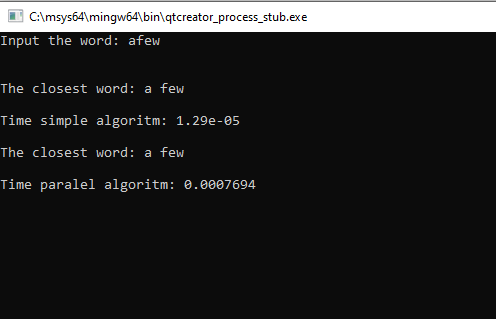
\includegraphics[scale=0.8]{../1.png}}
    \caption{Пример 1}
    \label{fig:image}
\end{figure}

\begin{figure}[h!]
    \center{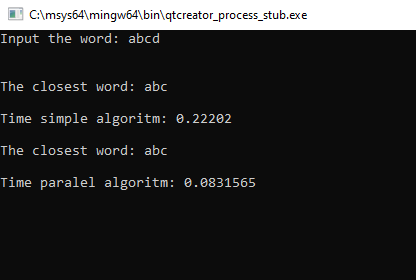
\includegraphics[scale=0.8]{../2.png}}
    \caption{Пример 2}
    \label{fig:image}
\end{figure}

Программа работает корректно.

\newpage
\section{Оценка времени}

Для замера процессорного времени исполнения функции используется функция 
QueryPerfomanceCounter библиотеки windows.h. \cite{}

Измерение производится в функциях, которые приведены в листинге 3.6.
 \\

\textrm{Листинг 3.6: функции замера процессорного времени}
\begin{lstlisting}[frame=single, numbers=left]
double PCFreq = 0.0;
__int64 CounterStart = 0;
    
void StartCounter()
{
    LARGE_INTEGER li;
    if(!QueryPerformanceFrequency(&li))
    std::cout << "QueryPerformanceFrequency failed!\n";
    
    PCFreq = double(li.QuadPart);///1000.0;
    
    QueryPerformanceCounter(&li);
    CounterStart = li.QuadPart;
}
    
double GetCounter()
{
    LARGE_INTEGER li;
    QueryPerformanceCounter(&li);
    return double(li.QuadPart-CounterStart)/PCFreq;
}
\end{lstlisting}

\section{Вывод}

Результатом технологической части стал выбор используемых технических средств 
реализации и последующая реализация алгоритмов и замера 
времени работы на языке C++.

\chapter{Исследовательская часть} 

Измерения процессорного времени проводятся на словарях c размерами: 
100, 1000, 10000, 100000. Средняя длина слова 7 букв.
Изучается серия экспериментов с количеством потоков 1, 2, 3, 4, 8, 16.

Для повышения точности, каждый замер производится 5 раз, за конечный результат 
берётся среднее арифметическое.

\section{Результаты экспериментов}

Эксперименты проводились на компьютере со следующими характеристиками:
\begin{itemize}
    \item ОС - Windows 10, 64bit;
    \item Процессор - Intel Core i3 7th Gen 2.3GHz, 2 Core 4 Logical Processor
    \item ОЗУ - 8Gb
\end{itemize}

По результатам измерений процессорного времени можно составить таблицы 4.1 - 4.4.

\begin{table}[h!]
\caption{Результаты замеров процессорного времени при размере 100 (в миллисекундах)}
\label{tabular:timesandtenses}
\begin{center}
\begin{tabular}{ | l | l | l | l | l | l | }
\hline
        Потоки                   & 1    & 2    & 4    & 8    & 16      \\ \hline
        Многопоточность  & 5.52 & 2.73 & 2.80 & 2.88 & 3.09  \\ \hline
        Однопоточно              &      \multicolumn{4}{c}{0.96}   &  \\ \hline
\end{tabular}
\end{center}
\end{table}

\begin{table}[h!]
\caption{Результаты замеров процессорного времени при размере 1000 (в секундах)}
\label{tabular:timesandtenses}
\begin{center}
\begin{tabular}{ | l | l | l | l | l | l | }
\hline
        Потоки                   & 1     & 2     & 4     & 8     & 16   \\ \hline
        Многопоточность & 0.0064 & 0.0054 & 0.0050 & 0.058 & 0.060 \\ \hline
        Однопоточно              &       \multicolumn{4}{c}{0.0051}       &       \\ \hline
\end{tabular}
\end{center}
\end{table}

\begin{table}[h!]
\caption{Результаты замеров процессорного времени при размере 10000 (в секундах)}
\label{tabular:timesandtenses}
\begin{center}
\begin{tabular}{ | l | l | l | l | l | l | }
\hline
        Потоки                   & 1    & 2    & 4    & 8    & 16    \\ \hline
        Многопоточность  & 0.037 & 0.025 & 0.012 & 0.012 & 0.014 \\ \hline
        Однопоточно              &     \multicolumn{4}{c}{0.032}    &      \\ \hline
\end{tabular}
\end{center}
\end{table}

\begin{table}[h!]
\caption{Результаты замеров процессорного времени при размере 100000 (в секундах)}
\label{tabular:timesandtenses}
\begin{center}
\begin{tabular}{ | l | l | l | l | l | l | }
\hline
        Потоки                   & 1    & 2    & 4    & 8    & 16    \\ \hline
        Многопоточность & 0.61 & 0.38 & 0.17 & 0.18 & 0.21 \\ \hline
        Однопоточно              &     \multicolumn{4}{c}{0.55}     &      \\ \hline
\end{tabular}
\end{center}
\end{table}

\newpage
\section{Вывод}

По результатам экспериментов можно заключить следующее:
\begin{itemize}
    \item при относительно небольшом размере словаря (менее 1000) использование потоков для 
    уменьшения времени исполнения нецелесообразно, так как накладные расходы времени на 
    управление потоками и mutex-ами больше, чем выигрыш от параллельного выполнения выполнения
    вычислений;
    \item использование по крайней мере двух потоков даёт ощутимый выигрыш по времени по 
    сравнению с однопоточной версией алгоритма;
    \item использование одного потока в многопоточных версиях алгоритма проигрывает по времени
    по сравнению с однопоточной версией алгоритма, что объясняется накладными расходами времени
    на управление потоками и mutex-ами;
    \item использование 8 и 16 потоков показывает результат по времени несколько хуже, чем при 
    4 потоках, из чего следует, что увеличение потоков даёт выигрыш по времени лишь до достижения
    определённого количества, так как появляются большие накладные затраты по времени для 
    управления большим количеством потоков и mutex-ов;
    \item наиболее быстродейственно алгоритм действует на 4 потоках, что равно количеству 
    логических процессоров на испытуемом компьютере.
\end{itemize}

\newpage
\chapter*{Заключение}
\addcontentsline{toc}{chapter}{Заключение} 

В ходе лабораторной работы достигнута поставленная цель: разработка и исследование алгоритма поиска наиболее похожего слова в словаре.
Решены все задачи.

Были описаны и реализованы непараллельная и параллельная реализации алгоритма.
Проведены замеры процессорного времени работы алгоритмов при различном количестве потоков.
На основании экспериментов проведён сравнительный анализ.

Из проведённых экспериментов было выявлено, что наиболее быстродеиственным является использование
количество потоков, которое совпадает с количеством логических процессоров процессора. 
Увеличение или уменьшение количества потоков ведёт к большему времени выполнения вычислений.
Однако, использование потоков даёт выигрыш по времени работы только для размеров словаря более 1000 записей, иначе их использование лишь увеличит время вычислений за счёт накладных
расходов.

\newpage
\renewcommand\bibname{Список литературы}
\addcontentsline{toc}{chapter}{Список литературы}
\makeatletter % список литературы
\def\@biblabel#1{#1. }
\makeatother
\begin{thebibliography}{4}
    \bibitem{cpp_info} Документация языка C++ 98 [Электронный ресурс], режим доступа: http://www.open-std.org/JTC1/SC22/WG21/, свободный (дата обращения: 14.10.2021).
    \bibitem{belous_off} R. A. Wagner, M. J. Fischer. The string-to-string correction problem. J. ACM 21 1 (1974). P. 168—173
    \bibitem{ll} В. И. Левенштейн. Двоичные коды с исправлением выпадений, вставок и замещений символов. Доклады Академий Наук СССР, 1965. 163.4:845-848.
    \bibitem{new} Mutex C++ $[$Электронный ресурс$]$.-Режим доступа: https://www.cplusplus.com/reference/mutex/mutex/ (Дата обращения 21.10.2021)
\end{thebibliography}

\end{document}